\subsection{Particle Filter}

The Particle Filter, implemented as Monte Carlo Localization (MCL), represents the belief state using a set of weighted samples and evaluates the Bayes filter equations \ref{eq:bayes_prediction} and \ref{eq:bayes_measurement_update} by Monte Carlo simulation \cite{thrun2005probabilistic}.

\subsubsection{Prediction}
The Particle Filter begins the prediction step by creating noise proportional to the velocity commands for each particle using Equations \ref{eq:v-noise} and \ref{eq:omega-noise}.
It also includes a noise floor value $\sigma_{\omega,\min}=0.02$ to maintain particle spread while the robot is stationary.
Random noisy movements are then injected into the particles using a normal distribution.

\begin{equation}
    \Delta d^i \sim \mathcal{N}(v \Delta t, \sigma_v^2 \Delta t)
\end{equation}

\begin{equation}
    \Delta \varphi^i \sim \mathcal{N}(\omega \Delta t, \sigma_\omega^2 \Delta t)
\end{equation}

These values are then converted into per-particle velocities.

\begin{equation}
    v^i = \frac{\Delta d^i}{\Delta t}
\end{equation}

\begin{equation}
    \omega^i = \frac{\Delta \varphi^i}{\Delta t}
\end{equation}

These velocities are then applied to each particle using the forward kinematics described in Equation \ref{eq:discrete_unicycle_kinematics}.
An illustration of the PF prediction algorithm can be found in Figure \ref{fig:pf_prediction}.

\begin{figure}[!htbp]
    \centering
    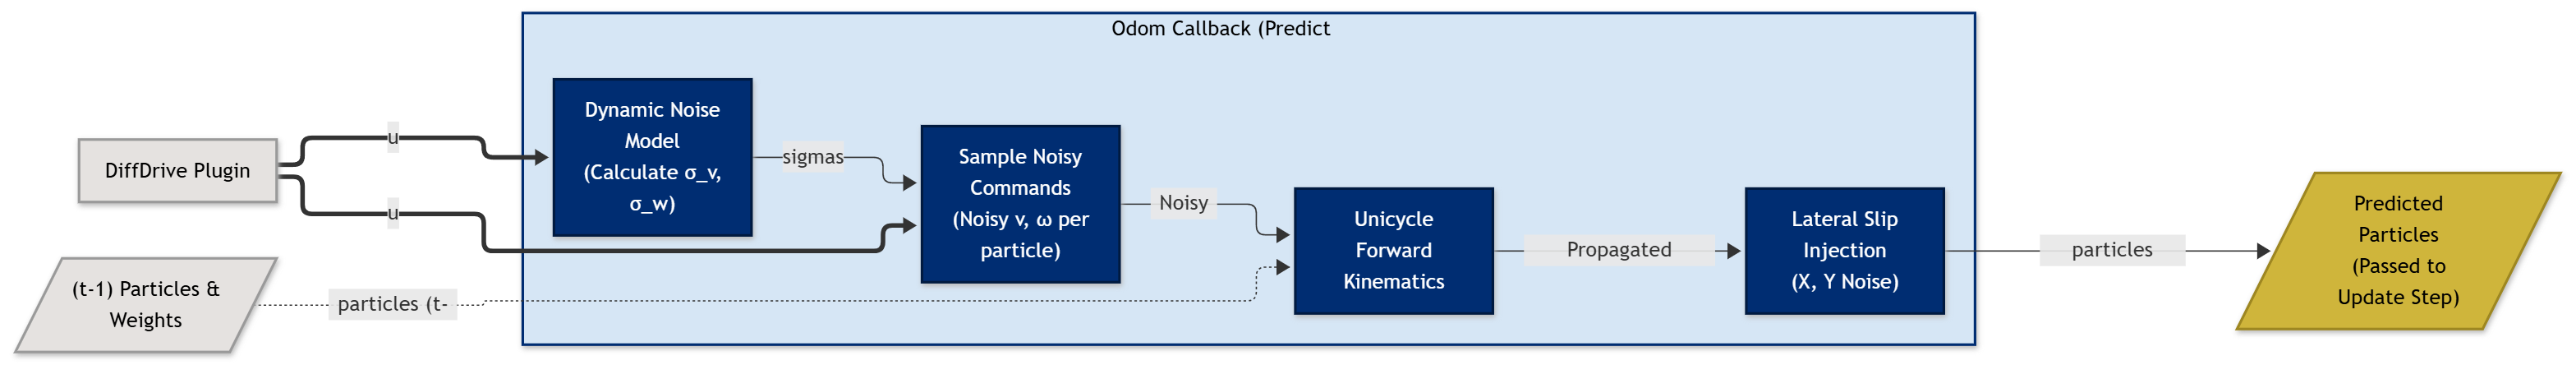
\includegraphics[width=\textwidth]{figures/pf_predict.png}
    \caption{Particle Filter Prediction Algorithm}
    \label{fig:pf_prediction}
\end{figure}

\subsubsection{Measurement Update}
The measurement step is illustrated in Figure \ref{fig:pf_update}.
The weight of each particle is updated using a Likelihood Field sensor model \cite{thrun2005probabilistic}. 
Rather than extracting a direct pose estimate from the scan like the EKF, the PF evaluates the raw LiDAR ranges against a pre-computed distance transform map found using SciPy \cite{scipyedt}. 
For a given particle pose hypothesis, each LiDAR endpoint $k$ is projected into the global map to find its Euclidean distance $d_k$ to the nearest obstacle. Assuming zero-mean Gaussian sensor noise with standard deviation $\sigma_{hit}$, the likelihood of a single beam is:
\begin{equation}
p(z_t^k \mid \mathbf{x}_t^{[m]}) \propto \exp \left( -\frac{d_k^2}{2\sigma_{hit}^2} \right)
\end{equation}
The total weight for particle $m$ is proportional to the product of the likelihoods of all valid beams. 
To prevent numerical underflow in floating-point operations, this is computed in log-space using the log-sum-exp trick:
\begin{equation}
w_t^{[m]} = \eta \exp \left( \sum_{k} \log p(z_t^k \mid \mathbf{x}_t^{[m]}) \right)
\end{equation}
where $\eta$ is a normalization constant ensuring that $\sum_{m=1}^M w_t^{[m]} = 1$.

\begin{figure}[!htbp]
    \centering
    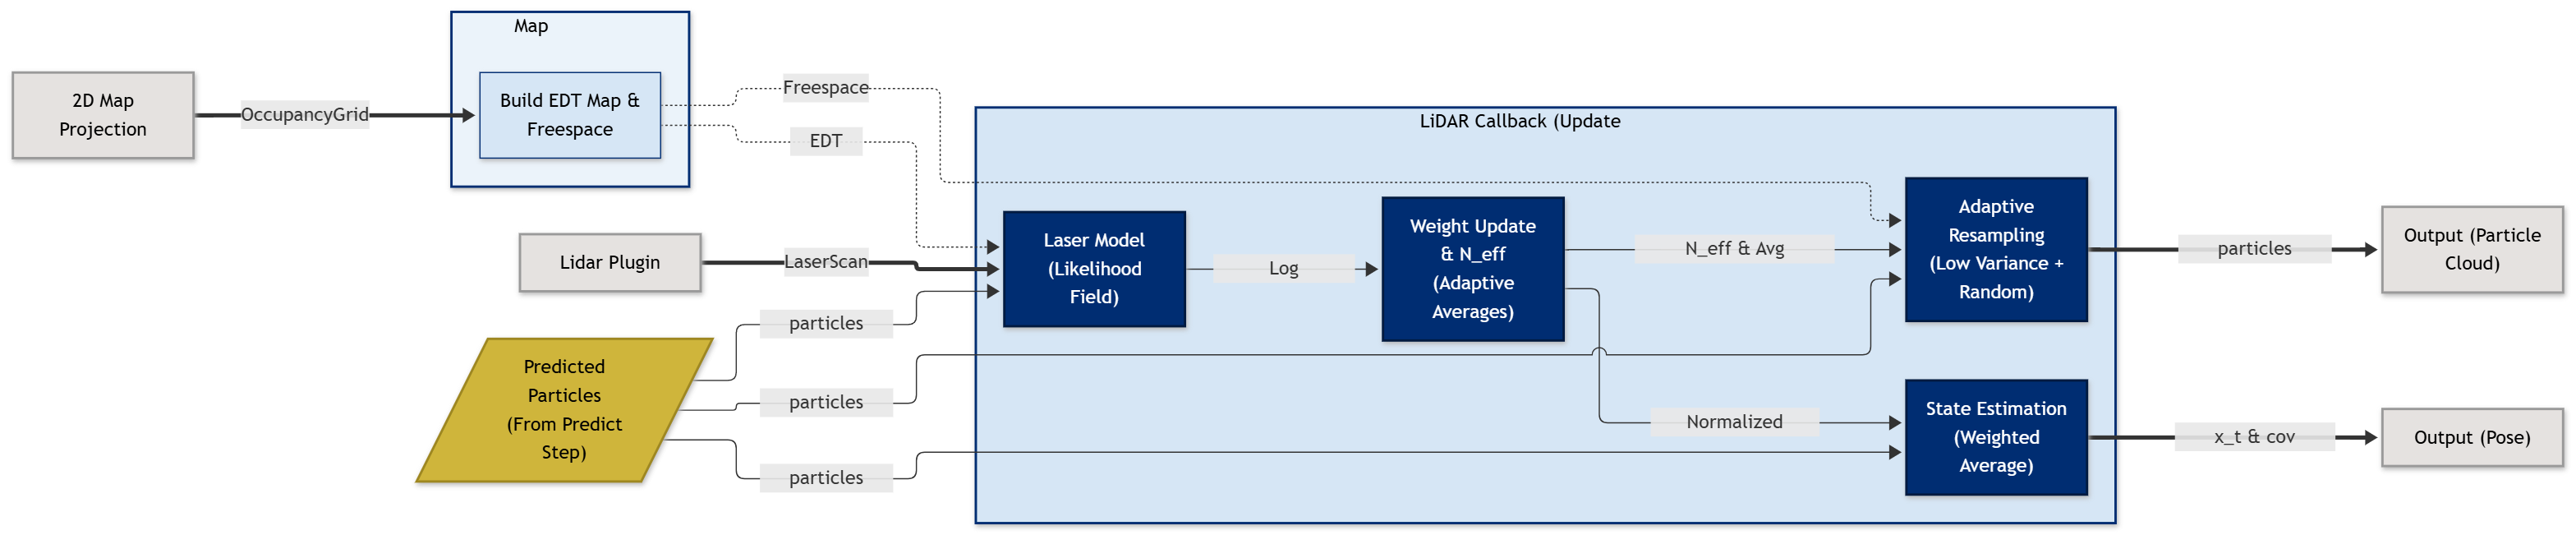
\includegraphics[width=\textwidth]{figures/pf_update.png}
    \caption{Particle Filter Update Algorithm}
    \label{fig:pf_update}
\end{figure}

\subsubsection{Resampling}
To prevent particle deprivation, where a majority of the computational effort is spent updating particles with near-zero weights, low-variance resampling is applied. 
A new set of $M$ particles is drawn from the current set with replacement, where the probability of drawing particle $m$ is proportional to its weight $w_t^{[m]}$. 
This focuses the distribution on the most probable regions of the state space.
The implementation of the PF node and algorithm can be found in Appendix \ref{subsec:PF implementation}.